\section{Benefits of Tiny Tasks}
\label{sec:benefits}
Tiny tasks benefit data center workloads by providing inherent elasticity:
fine-grained units of work can be dynamically allocated to machines as
resources become available, eliminating stragglers and issues of data skew,
and allow jobs to use available resources without sacrificing fairness
when new jobs are submitted.

\subsection{Inherent handling of skew and stragglers}
\paragraph{Data Skew}
Describe 3 types of skew (Josh). Tiny tasks turn a data partitioning problem into
a task scheduling problem. One graph comparing tiny tasks to skew partitioning
techniques.

\begin{figure}[t]
\centering
\hspace{2ex}
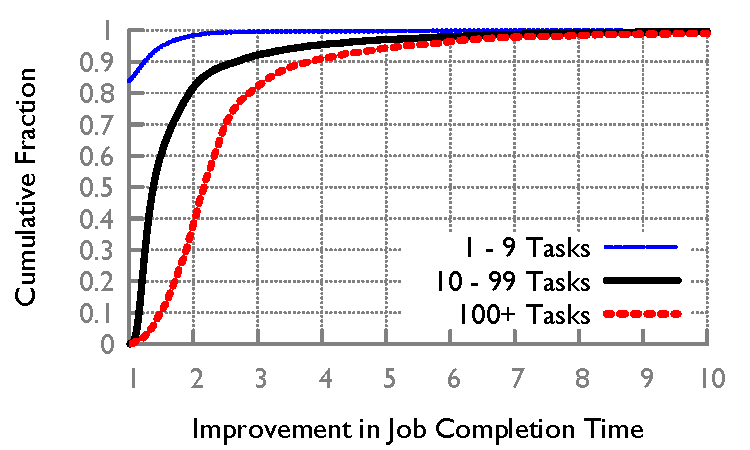
\includegraphics[width=0.5\textwidth]{figures/binpacked1-sep}
\vspace{-4ex}
\caption{Ideal improvement from binpacking tasks.}
\vspace{-2ex}
\label{fig:binpacked}
\end{figure}


\paragraph{Stragglers}
Reason for many stragglers unknown. Mantri paper attributes X\% of stragglers
to data skew, but the reason for the remaining ones is unknown. Tiny tasks
balance work over slaves, regardless of the reason for the skew.
Figure~\ref{fig:binpacked} demonstrates the improvement if we
balanced load across tasks perfectly.

\subsection{Fairness NEED A BETTER NAME}
Diagram here showing a before and after of what happens when a new job arrives
(and another job was already using the entire cluster)

Talk about Amoeba tradeoff.

Big win here is the ability seamlessly integrate batch and interactive workloads.

Simulation of response times for differently sized jobs as paralleism increases.

